\documentclass[letterpaper,10pt]{article}

\usepackage[english]{babel}
\usepackage[utf8]{inputenc}
\usepackage{amsmath}
\usepackage{graphicx}
\usepackage[colorinlistoftodos]{todonotes}
\usepackage[top=1in, bottom=1in, left=1in, right=1in]{geometry}
\usepackage[small]{titlesec}

\newcommand{\bes}{\begin{equation*}}
\newcommand{\ben}[1]{\begin{equation}\label{#1}}
\newcommand{\ees}{\end{equation*}}
\newcommand{\be}{\begin{equation}}
\newcommand{\ee}{\end{equation}}

\newcommand{\bm}[1]{% inline column vector
	\begin{bmatrix}#1\end{bmatrix}%
}

\begin{document}

\begin{flushright}
{\Large Josh Bevan - Midterm Q2 - CS556}
\end{flushright}
\vskip -0.1in
\hrule
\vskip 0.3in

\hskip -.3in{\large \textit{Consider the 200x200 diagonal matrix A, where diag(A) = (np.linspace(1,1000, 200)) and b=A1 (the vector of ones). Solve Ax=b with CG and BiCG}}

\section*{ How does BiCG's behavior compare to CG when you choose $ r^*_0=r_0$? Why? What about when $ r^*_0$ is something else?}
Figure 1 plots both the residuals and L2 errors for CG and BCG for when  $ r^*_0=r_0$, with $r_0$ being initialized to a random vector. The most noticeable comparison between them is that they give exactly the same results. This is unsurprising given the nature of the $\mathbf{A}$ matrix, which is symmetric positive definite. The symmetry means that $\mathbf{A}=\mathbf{A^T}$, so when BCG attempts to solve the matrix $\mathbf{B}$ it is actually just solving the same problem twice. The SPD nature of $\mathbf{A}$ leads to CG and BCG performing the same exact process. The result is they have identical convergence and error results.

\begin{figure}[!htb]
\centering
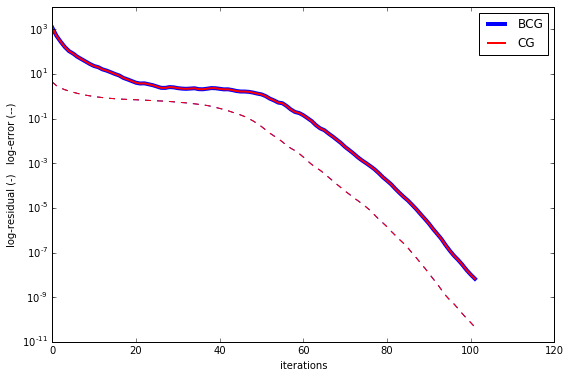
\includegraphics[width=1.05\textwidth]{k0VS.PNG}
\caption{Comparison between CG and BCG; k=0, $r^*_0 = r_0$}
\end{figure}

If instead we chose $r^*_0$ to be a different starting random vector, unique from $r_0$ we can observe the behavior in Figure 2. In contrast to Figure 1, BCG and CG do not have identical convergence behavior. For several example random starting vectors the same gross behavior was observed: residuals had similar but not identical convergence behavior with CG generally having a smaller residual that BCG at the same iteration number. The superior residual convergence of CG compared to BCG can perhaps be explained by it needing to only improve upon 1 starting random vector. In comparison BCG manipulates two separate vectors that are initialized at random; whichever residual currently is greater will cause the overall convergence to lag.

One other interesting feature to note in Figure 2 is that the L2 error for each method agrees much more closely. Consider that CG seeks to minimize the A-norm of the error. While BCG formally is not guaranteed to minimize anything, the fact that $\mathbf{A}=\mathbf{A^T}$ means BCG is attempting to solve a very similar problem to CG despite the fact that $r^*_0 \neq r_0$. In this respect we might expect BCG to display very similar error convergence behavior to CG, both of which should have a much more well behaved error convergence in contrast to residual convergence behavior. This may explain why the error curves agree so well for CG and BCG.

\begin{figure}[!htb]
\centering
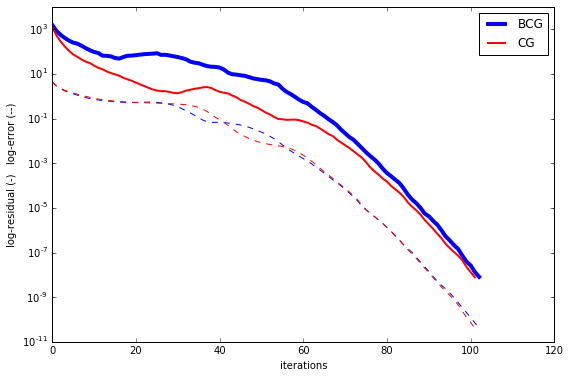
\includegraphics[width=1.05\textwidth]{k0VSrs.PNG}
\caption{Comparison between CG and BCG; k=0, $r^*_0 \neq r_0$}
\end{figure}

\section*{ Now consider $\mathbf{A_k}=\mathbf{A}-k\mathbf{I}$. What happens to BiCG convergence as k increases toward $k=50$? Why does this happen?}
Figures 3-5 compare values of k=10,30, and 50 respectively; there are two major features to note. First, there are a number of peaks in both the error and residual in the first half of iterations. Second, convergence is stagnant in general until shortly after the last of the peaks has been passed, after which the convergence rate is much greater.

If one examines the number of negative eigenvalues for each of the matrices it is apparent that it is the same as the number of peaks. The peaks are likely due to the difficulty in ``detecting'' these eigenvalues. A significant amount of iterations are necessary to find each of these modes, during which the residual and error are dominated by the contributions from the negative eigenvalues compared to the other eigenvalues and the gross convergence of the overall system is poor. After all of the negative eigenvalues are sufficiently included in the Krylov space BCG is able to converge much more rapidly and is no longer dominated by the negative eigenvalues. One major effect of this delayed convergence is that the same size system requires more iterations to reach the same tolerance level. Finally it is interesting to note that unlike the $k=0$ cases previously discussed the error is not necessarily guaranteed to be decreasing everywhere.

\begin{figure}[!htb]
\centering
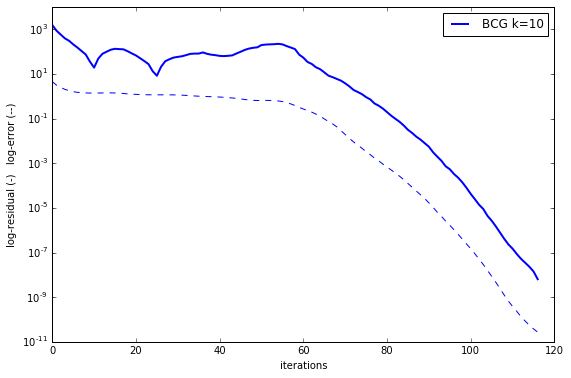
\includegraphics[width=0.6\textwidth]{BCG10.PNG}
\caption{Comparison between CG and BCG; k=10, $r^*_0 = r_0$}
\end{figure}
\begin{figure}[!htb]
\centering
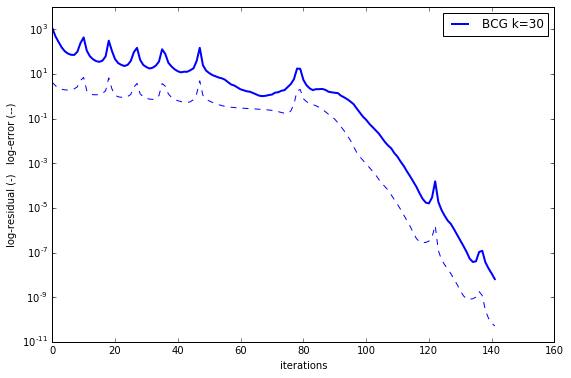
\includegraphics[width=0.6\textwidth]{BCG30.PNG}
\caption{Comparison between CG and BCG; k=30, $r^*_0 = r_0$}
\end{figure}
\begin{figure}[!htb]
\centering
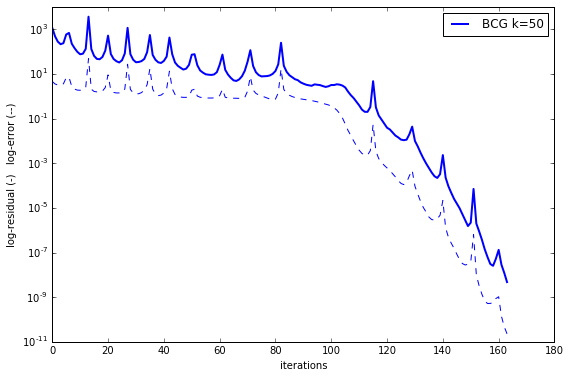
\includegraphics[width=0.6\textwidth]{BCG50.PNG}
\caption{Comparison between CG and BCG; k=50, $r^*_0 = r_0$}
\end{figure}

\clearpage

\section*{ Set $\mathbf{A_k}$ with $k=50$ and alter the last entry of $\mathbf{A}$ so that $\mathbf{A}[-1,-1]=1050$, making this last eigenvalue well-separated from the others, which are in [-49,950]. Look at r[4] and r[-1], the fifth and last components of the residual, and consider their convergence over 30 iterations. What do you notice?}

The last component of the residual converges much more rapidly than the 5th element (Figures 7 and 6, respectively), being several orders of magnitude smaller after 30 iterations. Also, the peaks that dominate r[4] are far less pronounced in r[-1].

This may be caused by there being a much larger component of the residual due to the negative eigenvalues present in r[4] compared to r[-1]. Interestingly, the fact that the component of the residual in r[-1] is already so small after 30 iterations shows that potentially BCG has already resolved most of the easier eigenvalues, but is hidden in the overall convergence rate by the negative eigenvalues' effects.

\begin{figure}[!htb]
\centering
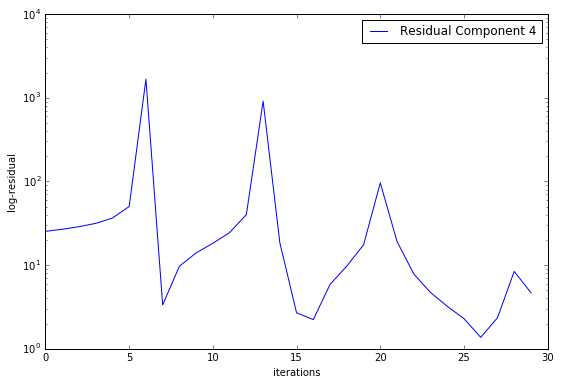
\includegraphics[width=0.6\textwidth]{r4.PNG}
\caption{Evolution of the 5th element of the residual for modified $A_k$}
\end{figure}
\begin{figure}[!htb]
\centering
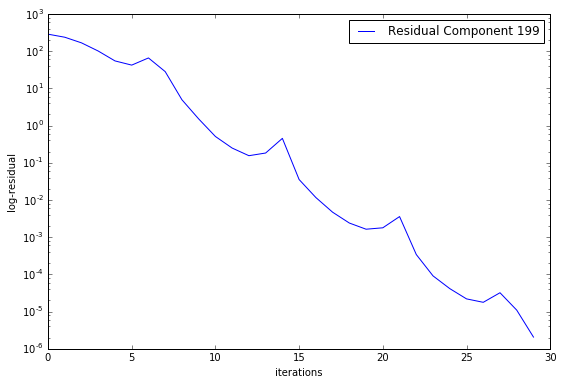
\includegraphics[width=0.6\textwidth]{rm1.PNG}
\caption{Evolution of the last element of the residual for modified $A_k$}
\end{figure}

\end{document}